\subsection{Összefoglaló feladatok}

\newcounter{feladatSzamlalo}

%_
\begin{frame}
  Fejlessze tovább a Wiki által ihletett, CSS-t ismertető weboldalt!
  \begin{columns}[c]
    \column{0.25\textwidth}
      \begin{exampleblock}{\textattachfile{cssFormazott.html}{cssFormazott.html}, \textattachfile{css.css}{css.css}}
        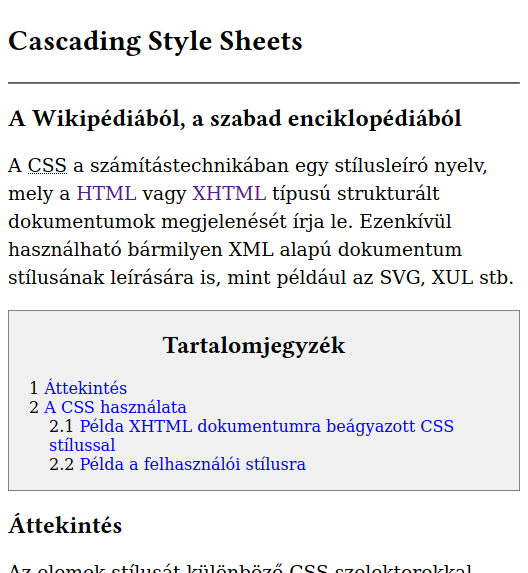
\includegraphics[width=\textwidth]{css1.png}
      \end{exampleblock}
    \column{0.75\textwidth}
      \begin{enumerate}
        \footnotesize
        \item Induljon ki a korábban létrehozott \textattachfile{../html2/css.html}{css.html} fájlból! Ha kell, egészítse ki a HTML kódot új (pl. \texttt{class}, \texttt{id}) attribútumokkal!
        \item Kapcsolja ezt össze egy \texttt{css.css} nevű stíluslappal, amit készítsen el az alábbi pontoknak megfelelően!
        \item A címsorok betűtípusa legyen \emph{Linux Libertine}, ennek hiányában \emph{Georgia}, \emph{Times}, de legalább valamilyen talpas betűkészlet!
        \item A bekezdések betűmérete legyen 14 nyomdai pont, a sortávolság legyen 1,5-szeres!
        \item Az első szintű címsor betűmérete legyen a bekezdések betűméretének 1,8-szerese, a második szintűké 1,5-szeres, a harmadik szintűeké pedig 1,2-szeres! Ez utóbbit szedje félkövér betűkkel!
        \item A hiperhivatkozások csak akkor legyenek aláhúzva, ha éppen felettük van az egér!
        \setcounter{feladatSzamlalo}{\theenumi}
      \end{enumerate}
  \end{columns}
\end{frame}

%_
\begin{frame}
  \begin{columns}[c]
    \column{0.25\textwidth}
      \begin{exampleblock}{\textattachfile{cssFormazott.html}{cssFormazott.html}, \textattachfile{css.css}{css.css}}
        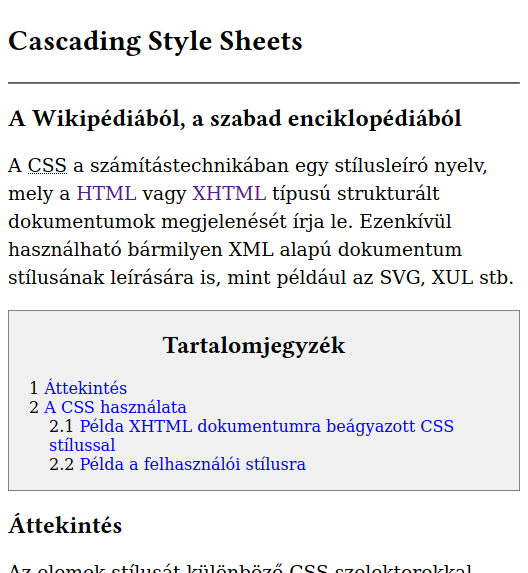
\includegraphics[width=\textwidth]{css1.png}
      \end{exampleblock}
    \column{0.75\textwidth}
      \begin{enumerate}
        \setcounter{enumi}{\thefeladatSzamlalo}
        \item A tartalomjegyzéket vegye körül 1 képpont széles, folytonos, szürke színű szegéllyel!
        \item A háttérszín is legyen szürke, melynek minden RGB komponense 240 értékű!
        \item Maga a tartalomjegyzék ne legyen szélesebb, mint amit a tartalma indokol!
        \item A jobb oldalon állítsa 20 képpontra a kitöltést!
        \item A ,,Tartalomjegyzék'' felirat legyen középre igazítva!
        \item A felsorolások bal oldali kitöltése legyen 20 képpont!
        \item A számozás szintenként folytonos legyen, a minta szerint!
        \setcounter{feladatSzamlalo}{\theenumi}
      \end{enumerate}
  \end{columns}
\end{frame}

%_
\begin{frame}
  \begin{columns}[c]
    \column{0.25\textwidth}
      \begin{exampleblock}{\textattachfile{cssFormazott.html}{cssFormazott.html}, \textattachfile{css.css}{css.css}}
        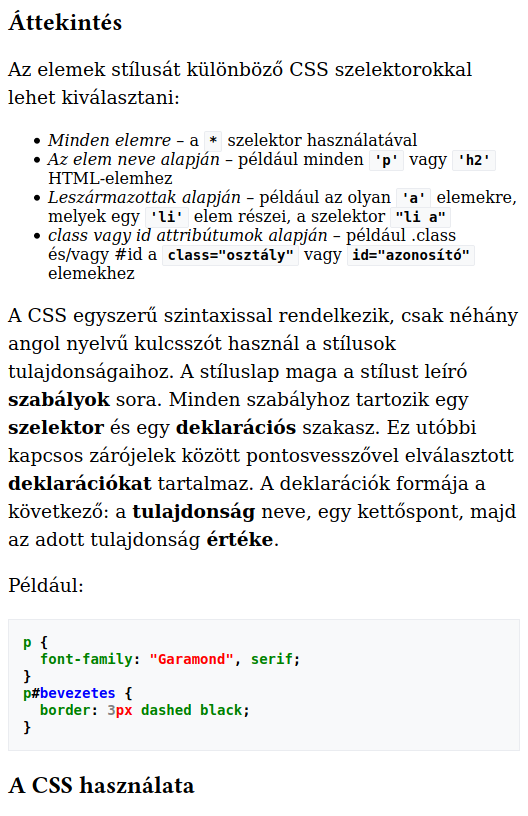
\includegraphics[width=\textwidth]{css2.png}
      \end{exampleblock}
    \column{0.75\textwidth}
      \begin{enumerate}
        \setcounter{enumi}{\thefeladatSzamlalo}
        \small
        \item A programkódok, akár egy soron belül helyezkednek el, akár előformázott szövegként, kapjanak világosszürke hátteret, melynek RGB összetevői 16-os számrendszerben rendre \texttt{f8}, \texttt{f9} és \texttt{fa}!
        \item A szegélyek 1 képpont széles, folytonos vonalak, melyek színének komponensei: \texttt{ea}, \texttt{ec} és \texttt{f0}!
        \item A szöveg legyen 14 képpont méretű, félkövér betűkkel szedett!
        \item Ha a kód soron belül található, a szegélye legyen 2 képpont sugarú lekerekítéssel ellátva, továbbá fent és lent 1-1, a két oldalon pedig 4-4 képpont belső kitöltéssel rendelkezzen!
        \item Ezzel szemben az előformázott szövegeknek minden oldalán hagyjon akkora kitöltést, mint amekkora az alapértelmezett betűméret!
        \setcounter{feladatSzamlalo}{\theenumi}
      \end{enumerate}
  \end{columns}
\end{frame}

%_
\begin{frame}
  \begin{columns}[c]
    \column{0.25\textwidth}
      \begin{exampleblock}{\textattachfile{cssFormazott.html}{cssFormazott.html}, \textattachfile{css.css}{css.css}}
        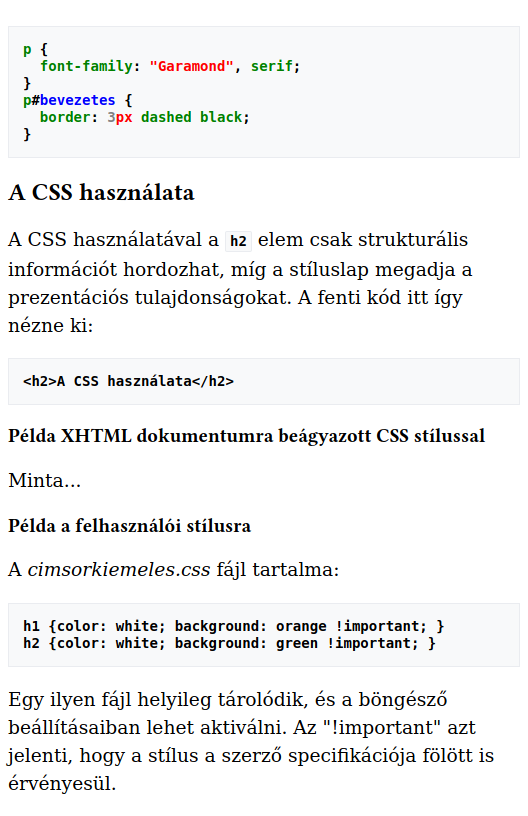
\includegraphics[width=\textwidth]{css3.png}
      \end{exampleblock}
    \column{0.75\textwidth}
      A szintaktikai kiemeléssel ellátott CSS forrásszövegben
      \begin{enumerate}
        \setcounter{enumi}{\thefeladatSzamlalo}
        \item az elemnevek, tulajdonságok és kulcsszavak színe legyen zöld,
        \item az \texttt{id} legyen kék,
        \item a mértékegység és a karakterlánc típusú adat legyen piros,
        \item a mennyiség pedig szürke!
      \end{enumerate}
  \end{columns}
\end{frame}
